The intent of this section is to define and justify the algorithms we have chosen to test in our research, additionally,
we can use preliminary tests of each algorithm as a baseline for their respective energy footprints in the Implementation
chapter.

\subsubsection{Experimental Space}
To prevent bias in specific operations, this paper will attempt to use a variety of scripts that perform different
purposes.
As a time constraint, the scripts should be simple to execute, and ideally should have very little ambiguity on their
intended execution - as an example, python libraries will not be considered, as they perform many functions, and it is
difficult to determine an execution path without a full understanding of the library.
Consequently, programs that operate on a resource, or connect to the internet will also not be considered, to prevent
time wasted on debugging network issues or misunderstandings of the operable resource.

Constraining the experimental space like this introduces an obvious bias, this can be addressed in continuations of this
research by expanding the experimental space to include more complex scripts.

The most obvious approach is to start by running benchmarks, as they are often designed to test the limits of a system
and are likely to explore a wide range of operations to draw conclusions.
For this report we will use the scripts defined in the Debian computer languages benchmark game\cite{BenchmarkGame}.
Relying on benchmarks has two major drawbacks: the first is that benchmarks necessarily are not a good representation
of a typical use case of a system, rather a way to expose the flaws of the tested system; the second issue is that
benchmarks must be designed to be comparable across the tested systems - in our case this means that all the algorithms
we have taken from the benchmark games were chosen for their broad applicability and may not cover a sufficient amount
of Python constructs to be useful for our purposes.
Nevertheless, the benchmarks will provide a good starting point for our research.
In a parallel approach, we can find example code to benchmark specific sectors by searching for research papers
comparing technologies in that sector, this provides a more focused approach to targeting specific concepts in Python,
as sufficiently well presented papers will provide control groups to eliminate technology bias.

We will attempt to keep algorithms at a baseline of 10 minute runs, this duration is chosen simply for convenience, as
it is short enough to run multiple times, and long enough to aid visual analysis of the data.
Each experiment will be run 10 times, to inspect variance in run time and energy usage, outliers will be identified by
unexplained rises in temperature, or large deviation from the mean.

\subsubsection{Sleep}
The most trivial process to profile is the sleep command, profiling a sleeping python script should give us a good
baseline for the energy usage of the python interpreter, and the footprint of the various profiling tools.

As can be seen in fig~\ref{fig:sleep_repeating}, the python interpreter has a completely negligible energy impact, and
can not be distinguished from the noise of the system.
For this reason, when forecasting future results, we can ignore baseline costs.

\begin{figure}[H]
    \centering
    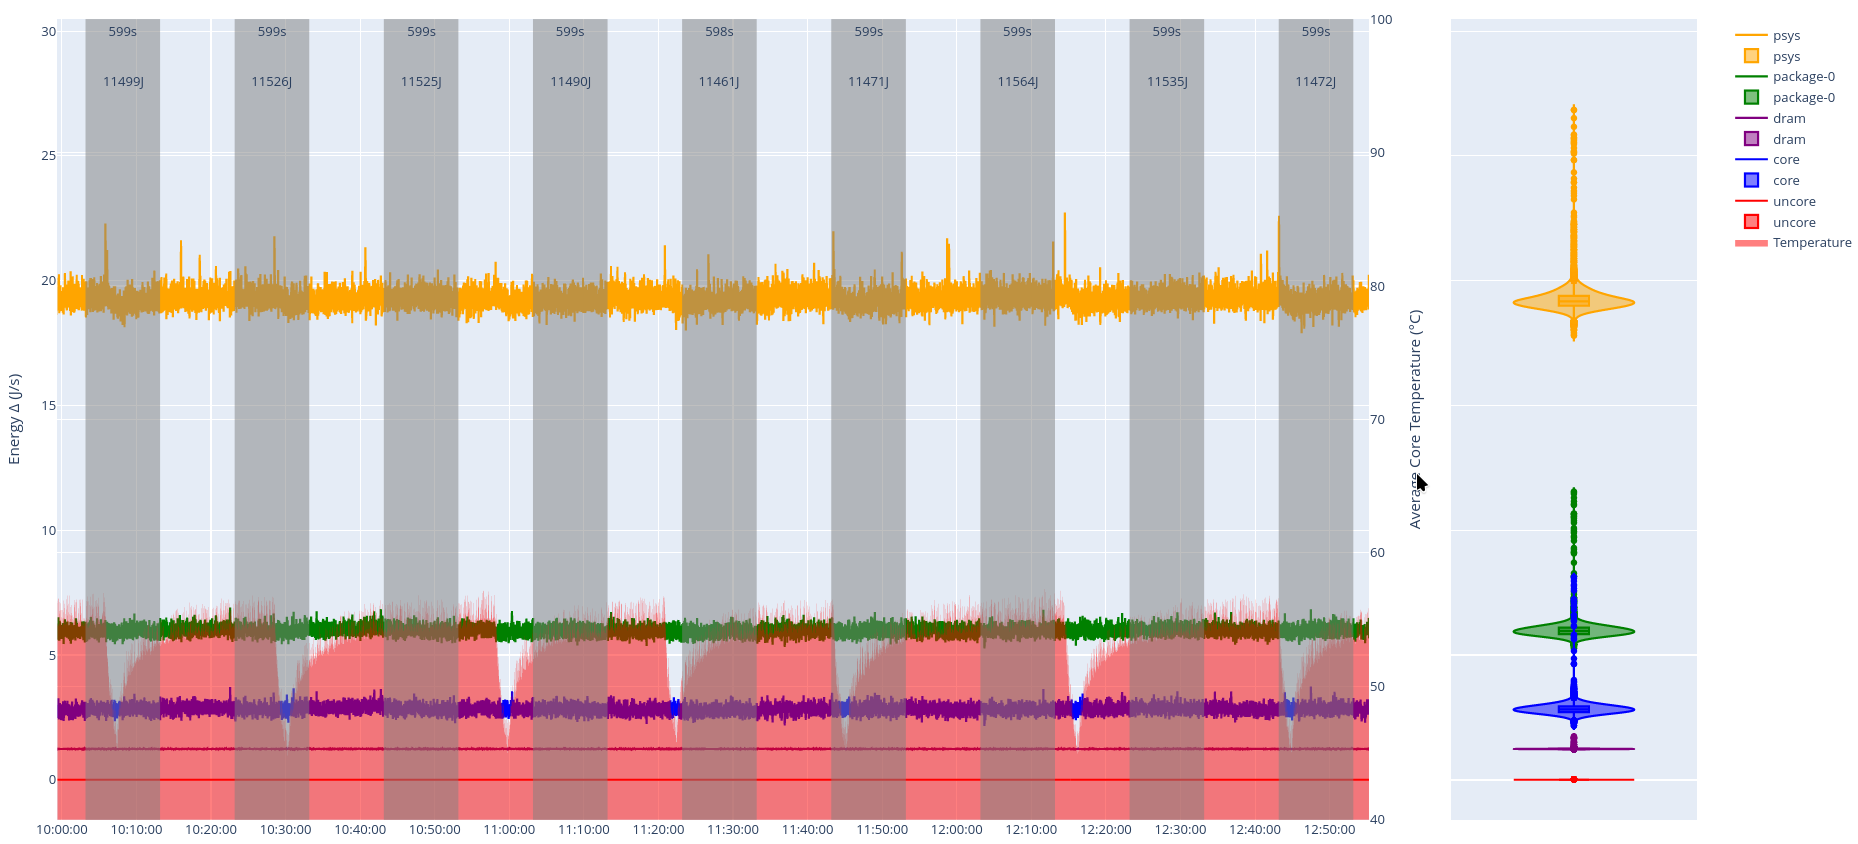
\includegraphics[width=15cm]{figures/implementation/sleep_repetition}
    \caption{Running sleep within python for 10 minutes, experiment durations are highlighted in grey}
    \label{fig:sleep_repeating}
\end{figure}

\textbf{Bash Time}
The sleep command is important for understanding the bash profiling tool, as we can see that sleeping has no visible
effect on overall power consumption, we will attempt to make the assumption that when bash profiling, time not spent in
usr or sys accounts for zero energy usage.
This assumption is likely incorrect, as simply executing the script will incur an energy cost, however we believe that
the value is low enough that it can be safely ignored.

\subsubsection{N-Body}
The n-body problem is a classic problem in physics, and is used to simulate the motion of celestial bodies in a system.
In order to come close to the 10-minute testing time that we have previously implemented for sleep, we are running this
algorithm with an input of 50 million.
As seen in~\ref{fig:nbody_repeating}, the algorithm is running at an average of 652 seconds, which is acceptably close
to the 10-minute mark, with an average of 15211 joules of energy used.
Visual analysis of the graph shows that energy usage varies highly (with a range of 13448 to 17119 joules), though this
seems to be directly proportional to the variance of time - this suggests that more promising results will be seen from
approaches that test for time, rather than the actual execution of the script.

\begin{figure}[H]
    \centering
    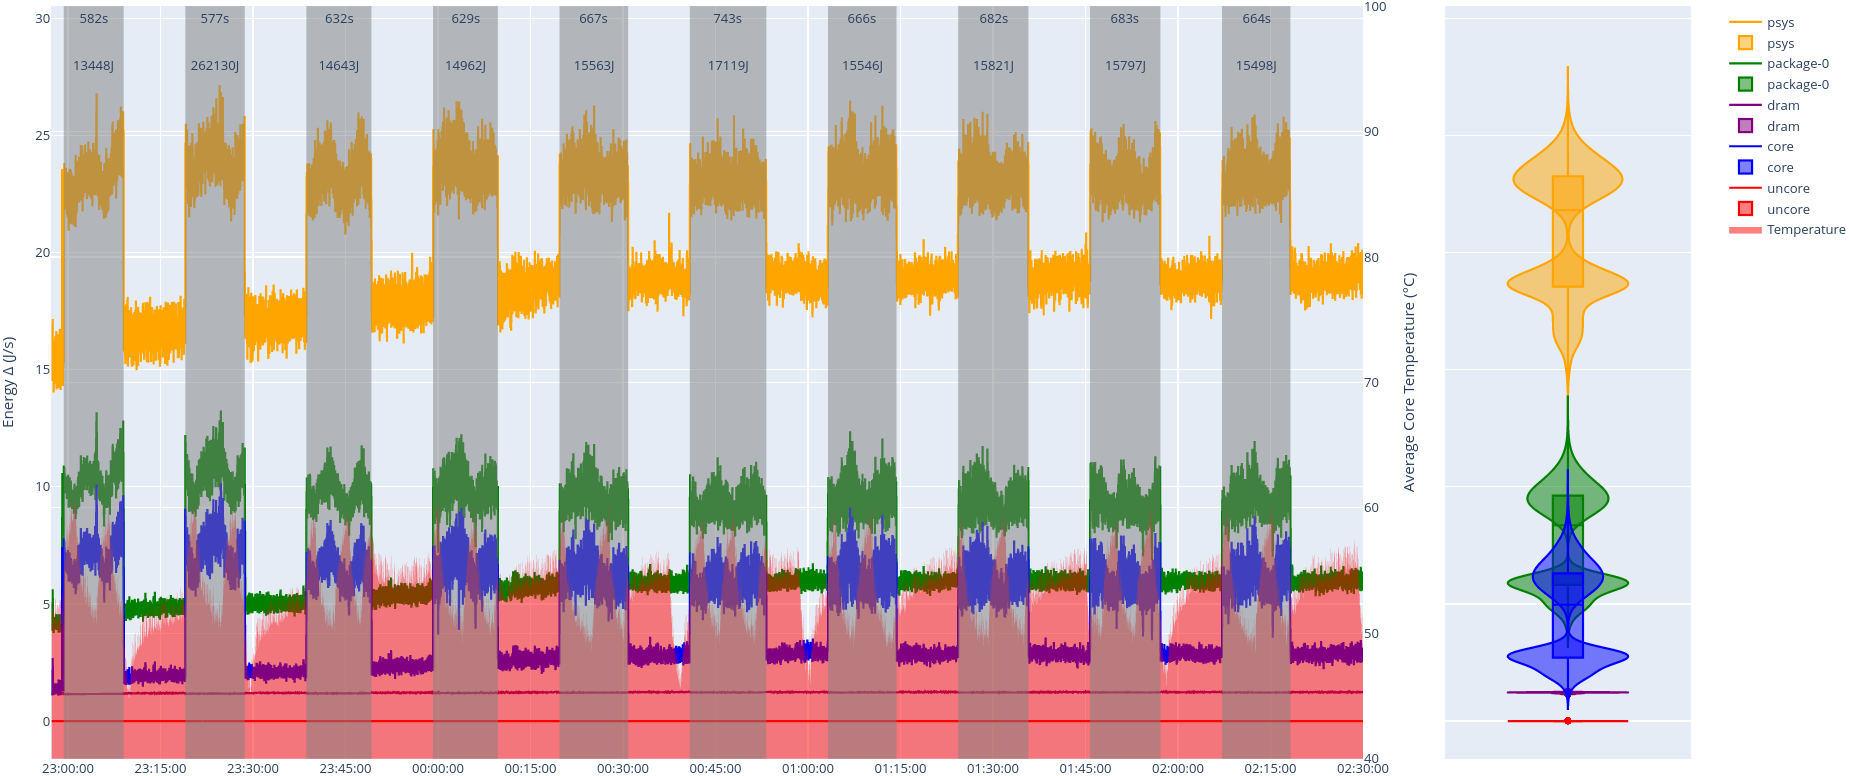
\includegraphics[width=15cm]{figures/implementation/nbody_repeating}
    \caption{Running the n-body problem, experiment durations are highlighted in grey}
    \label{fig:nbody_repeating}
\end{figure}

\textbf{Bash Time}
The n-body problem is a good example of a pure user space script, after 10 runs the mean of each time is as follows:
\textbf{real} - \textit{10m:48s} (std - 55s)
\textbf{user} - \textit{10m:48s} (std - 55s)
\textbf{sys} - \textit{0.02s} (std - 0.01s)

\subsubsection{Binary Trees}
Binary trees are a simple data structure that are classically used to as an excercise in computer science - for this
experiment we have specifically chosen an implementation that avoids multithreading, as we are interested in having
multiple algorithms that are sequential.
As seen in~\ref{fig:btree_repeating}, the algorithm is running at an average of 457 seconds, with an average energy
usage of 10860 Joules, this is a promisingly close result to the n-body problem (an average of 23.3J/s compared to
23.8J/s), and suggests that the energy usage of the python interpreter is consistent across different sequential
algorithms.


\begin{figure}[H]
    \centering
    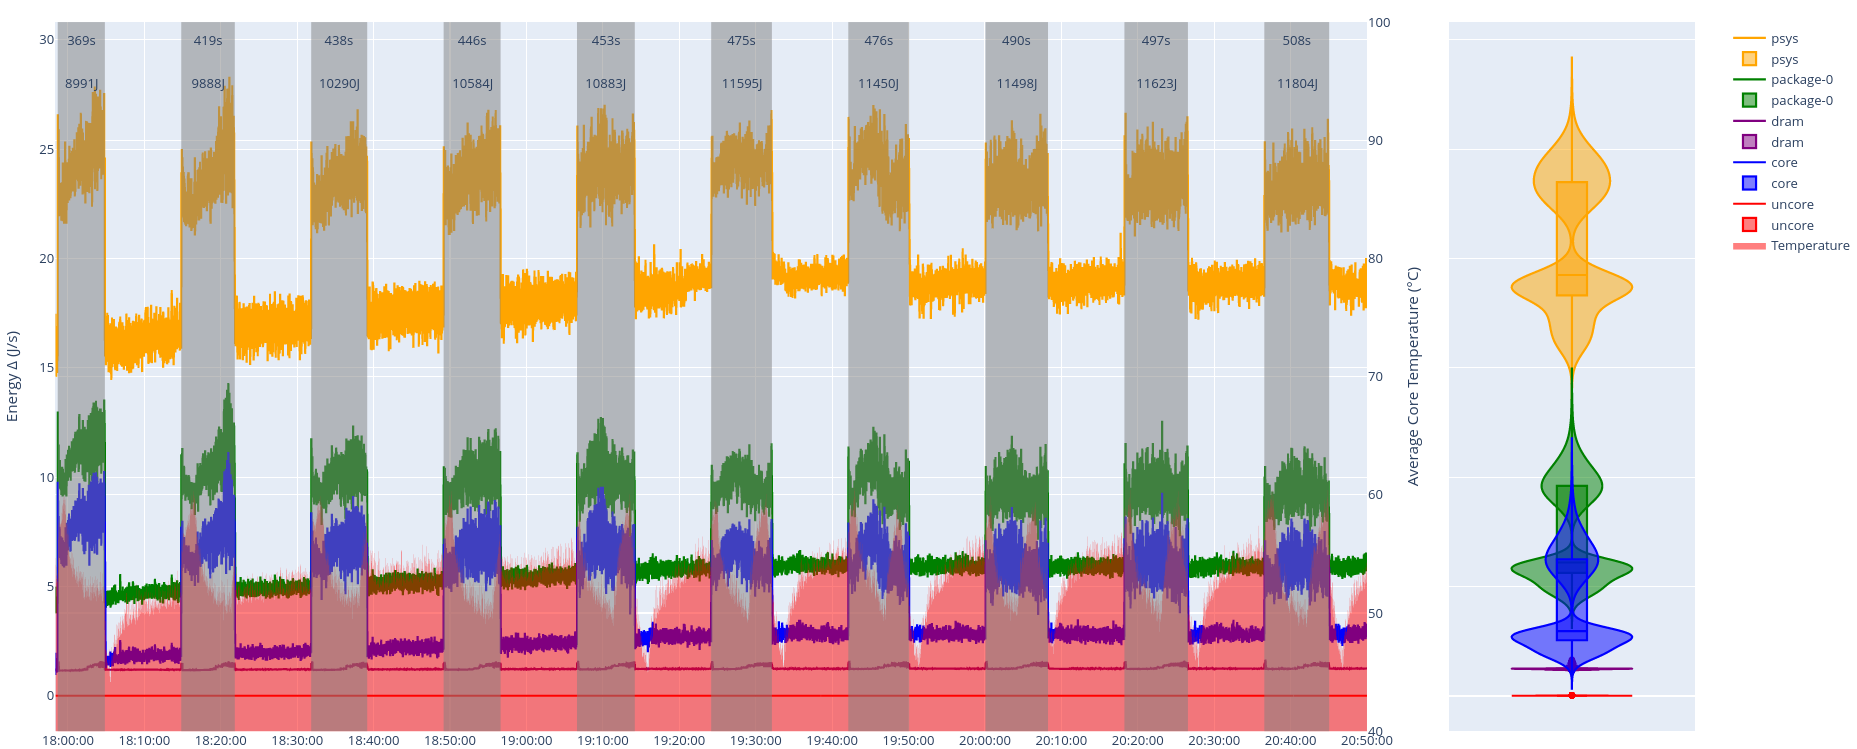
\includegraphics[width=15cm]{figures/implementation/btree_repeating}
    \caption{Running the binary tree algorithm, experiment durations are highlighted in grey}
    \label{fig:btree_repeating}
\end{figure}

\subsubsection{Mandelbrot}
Mandelbrot is a classic algorithm used to generate fractal images, and is often used as a benchmark for performance, we
have chosen this specific implementation as it is highly multithreaded, as can be seen in~\ref{fig:mandelbrot_repeating},
the core and package-0 domains are not only far lower than previous sequential algorithms, they are also far more stable;
this suggests that further research must be done to understand how the energy usage of multithreaded applications
affect energy usage.

In our preliminary experiments, the Mandelbrot algorithm has shown to execute at an average execution time of 585
seconds, with an average energy usage of 13341 Joules (averaging 22.8J/s).

\begin{figure}[H]
    \centering
    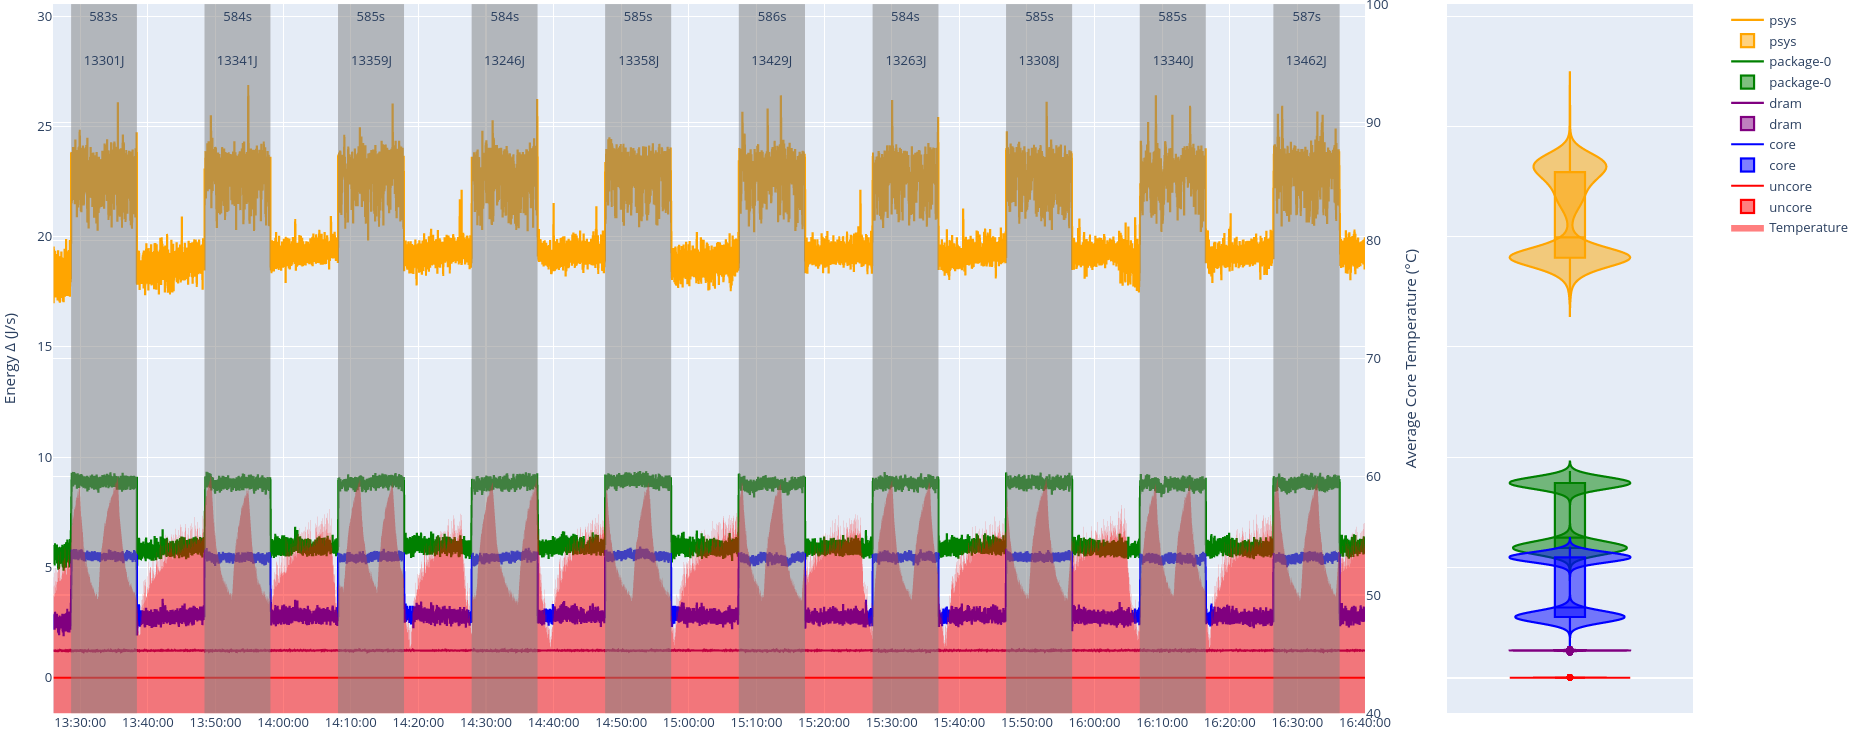
\includegraphics[width=15cm]{figures/implementation/mandelbrot_repeating}
    \caption{Running the mandelbrot algorithm, experiment durations are highlighted in grey}
    \label{fig:mandelbrot_repeating}
\end{figure}

\subsubsection{DataFrame Tester}
Python DataFrames are a powerful tool used for data manipulation and analysis, and is being used extensively to generate
the data seen in this report, we believe that DataFrame benchmarking is a useful avenue as they are often heavily
involved in running underlying C binaries, together with the fact that there may be some level of multithreading
implemented.
For this experiment we have found an article looking to compare and benchmark the performance of different dataframe
libraries~\cite{DataframeBenchmark} - unfortunately two of the four benchmarking libraries were too cumbersome to
implement, this is ultimately not an issue as the validity of the test is not a concern of this report.

As seen in~\ref{fig:dataframe_repeating}, the algorithm is running at an average of 217 seconds, with an average energy
usage of 5200 Joules, unfortunately, it has been difficult to find an input to reach an average 10-minute mark.

\begin{figure}[H]
    \centering
    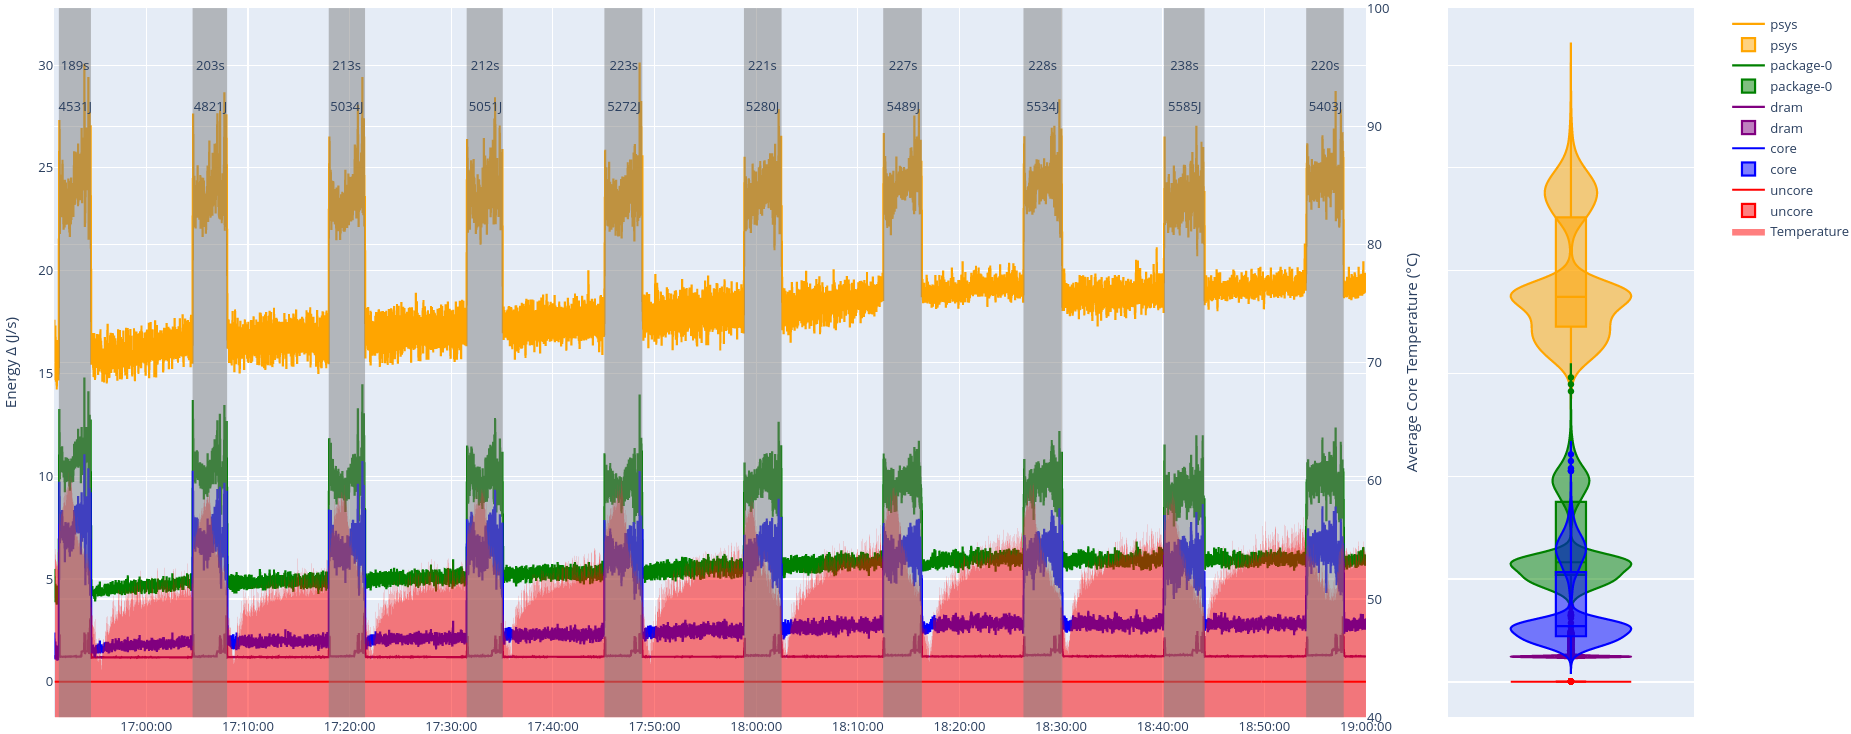
\includegraphics[width=15cm]{figures/implementation/dataframe_repetition}
    \caption{Running the dataframe tester, experiment durations are highlighted in grey}
    \label{fig:dataframe_repeating}
\end{figure}

\textbf{Bash Time}
The DataFrame tester brings two facets, firstly, the real time is lower than the sum of user and sys time, this
indicates that the process must be multithreaded - when looking at the sleep experiment, we suggested that time spent
outside the user and sys time would incur zero energy cost, while this experiment suggests that it might be
pertinent to ignore the value completely.

The statistics of the exploratory run are as follows:
\textbf{real} - \textit{3m:37s} (std - 15s)
\textbf{user} - \textit{5m:9s} (std - 14s)
\textbf{sys} - \textit{44s} (std - 1.5s)

